%%%%%%%% ICML 2026 SUBMISSION FILE %%%%%%%%%%%%%%%%%

\documentclass{article}

% Recommended packages
\usepackage{microtype}
\usepackage{graphicx}
\usepackage{subcaption}
\usepackage{booktabs}
\usepackage{hyperref}

\newcommand{\theHalgorithm}{\arabic{algorithm}}

% Blind submission
\usepackage{icml2026}
% For preprint:
% \usepackage[preprint]{icml2026}
% For camera-ready:
% \usepackage[accepted]{icml2026}

% Math packages
\usepackage{amsmath}
\usepackage{amssymb}
\usepackage{mathtools}
\usepackage{amsthm}

\usepackage[capitalize,noabbrev]{cleveref}

%%%%%%%%%%%%%%%%%%%%%%%%%%%%%%%%
% THEOREMS
%%%%%%%%%%%%%%%%%%%%%%%%%%%%%%%%
\theoremstyle{plain}
\newtheorem{theorem}{Theorem}[section]
\newtheorem{proposition}[theorem]{Proposition}
\newtheorem{lemma}[theorem]{Lemma}
\newtheorem{corollary}[theorem]{Corollary}
\theoremstyle{definition}
\newtheorem{definition}[theorem]{Definition}
\newtheorem{assumption}[theorem]{Assumption}
\theoremstyle{remark}
\newtheorem{remark}[theorem]{Remark}

\icmltitlerunning{FORGE: Real-World Generative Engineering Evaluation}
\usepackage{tikz}
\usetikzlibrary{arrows.meta,positioning}
\usepackage{pgfplots}
\pgfplotsset{compat=1.18}

\begin{document}

\twocolumn[
\icmltitle{FORGE: A Framework for Real-World Generative Engineering Evaluation of AI Agents}
]
\icmlcorrespondingauthor{Anonymous Author}{anonymous@icml.cc}
\printAffiliationsAndNotice{}  % Required, keep empty for blind review

% =========================
% Abstract
% =========================
\begin{abstract}
Existing benchmarks frequently overestimate the capabilities of AI agents by evaluating isolated code snippets rather than holistic system construction. They often fail to assess whether an agent can construct a functional, integrated system. We introduce \textbf{FORGE}, a comprehensive framework that requires agents to engineer complete software projects. FORGE executes generated artifacts within \textbf{Isolated Processes} and an \textbf{Essential Sandbox} to assess functional viability, stability, and error recovery. Our evaluation reveals a significant divergence: models proficient in generating isolated snippets frequently fail to construct integrated projects. FORGE provides a rigorous assessment of agent readiness for real-world software engineering tasks.
\end{abstract}


% =========================
% Main Paper
% =========================
\section{Introduction}

Recent advancements in AI have yielded models proficient in code generation. However, prevailing evaluations predominantly assess the ability to synthesize single functions or pass isolated tests. In professional engineering contexts, code synthesis constitutes merely the initial phase; file organization, execution management, and stability assurance are equally critical.

Consequently, models achieving high scores on existing benchmarks often fail to construct functional systems. A dichotomy exists between passing unit tests and fulfilling real-world specifications. We posit that AI should be evaluated on its capacity to deliver functional software.

This premise is grounded in the view that intelligence manifests through interaction with the environment rather than abstract reasoning alone. Utility is defined by an agent's ability to utilize tools, manage constraints, and rectify errors. While in-context learning is not the primary focus, the ability to handle runtime exceptions—such as compiler warnings or crashes—and maintain continuity is essential. Software engineering entails the delivery of executable deliverables, not merely syntactically correct text.

Many contemporary benchmarks rely on comparing generated code to a canonical solution. While facilitating automated grading, this approach often overlooks the broader engineering context. Such evaluations rarely require models to manage multi-file architectures, resolve dependencies, or execute code. Consequently, they provide limited insight into a model's ability to construct functional software.

Passing unit tests does not guarantee system viability, as unit tests are inherently simplified and isolated. Real-world projects frequently fail due to structural deficiencies, missing artifacts, or logical inconsistencies, even when individual components are correct.

To address these limitations, we developed \textbf{FORGE}. FORGE evaluates agents on realistic engineering tasks, moving beyond text analysis to require the construction and execution of complete projects. The model receives system feedback, such as error logs, and must handle these signals. This approach allows for the assessment of structural integrity and runtime viability. FORGE aims to bridge the gap between benchmark performance and practical engineering capability.

This paper makes three primary contributions. First, it formalizes real-world testing into a quantifiable metric. Second, it establishes a rigorous methodology for assessing project structure and runtime behavior. Third, it provides a standardized task suite and a failure taxonomy to facilitate the analysis of agent failure modes. These tools enable the evaluation of AI reliability and consistency.

\section{Related Work}

We review prior work on evaluating AI coding capabilities. Existing benchmarks generally fall into three categories: unit-test benchmarks, agent tool-use evaluations, and engineering-oriented benchmarks.

\paragraph{Unit-test benchmarks.}
These benchmarks assess a model's ability to generate a single function that satisfies a test case. Datasets such as HumanEval and MBPP are widely adopted due to the ease of automated evaluation \cite{humaneval,mbpp,apps}. However, they primarily evaluate isolated code snippets and do not assess the ability to construct complete projects or manage dependencies. Success in these benchmarks does not necessarily imply the capability to engineer runnable software. FORGE addresses this limitation by evaluating full project construction rather than isolated snippets.

\paragraph{Agent and tool-use tests.}
Several benchmarks evaluate how agents utilize tools. Benchmarks like AgentBench and WebArena assess an agent's ability to follow plans or navigate the web \cite{agentbench,webarena,toolllm,gaia}. While valuable, these benchmarks often focus on task completion rates without deeply analyzing failure modes or execution stability. FORGE generates a detailed report of execution failures, providing granular insight into the causes of failure.

\paragraph{Engineering benchmarks.}
Recent benchmarks such as SWE-bench attempt to increase realism by asking models to resolve issues in existing codebases \cite{swebench}. Others examine how agents interact with code repositories \cite{sweagent,repobench}. While these represent an improvement, they focus primarily on bug fixing and often rely on binary pass/fail metrics without explanatory detail. FORGE encompasses a broader range of tasks—including greenfield project creation—and provides a systematic taxonomy for categorizing failures.

In summary, earlier benchmarks tend to focus on code snippets or binary outcomes. FORGE fills this gap by testing whether an agent can construct a runnable software project within a realistic environment.
\section{Method}

\subsection{Problem Statement}
This section delineates the distinction between FORGE and traditional benchmarks.

\begin{definition}[Static Patch Evaluation $B_{SWE}$]
A benchmark that evaluates agents based on the ability of a code patch to satisfy a verification suite. It operates within a static context and does not mandate the delivery of a comprehensive product, iterative error resolution, or execution within a realistic environment.
\end{definition}

\begin{definition}[In-field Project Evaluation $B_{FORGE}$]
A project-based benchmark evaluating agents via the execution of a comprehensive workflow under defined constraints. Agents are required to construct functional software, with success quantified by runtime performance and production cost.
\end{definition}

\begin{proposition}[Evaluation Order Mismatch]
For a significant subset of agents, the ranking derived from field evaluation consistently diverges from that of static evaluation:
\begin{equation}
\text{Rank}(B_{FORGE}) \neq \text{Rank}(B_{SWE})
\end{equation}
\end{proposition}

\subsection{FORGE Framework Overview}

\begin{figure}[t]
\centering
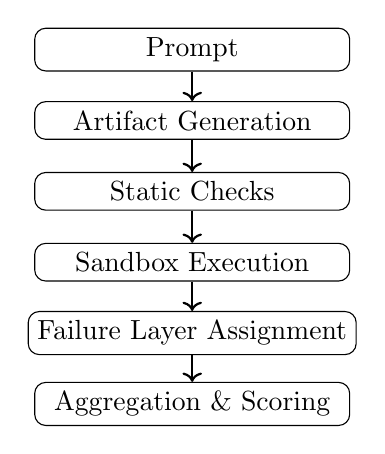
\begin{tikzpicture}[
  node distance=0.9cm,
  every node/.style={
    draw, rectangle, rounded corners,
    align=center, minimum width=4cm
  },
  arrow/.style={->, thick}
]

\node (prompt) {Prompt};
\node (gen) [below of=prompt] {Artifact Generation};
\node (static) [below of=gen] {Static Checks};
\node (exec) [below of=static] {Sandbox Execution};
\node (fail) [below of=exec] {Failure Layer Assignment};
\node (agg) [below of=fail] {Aggregation \& Scoring};

\draw[arrow] (prompt) -- (gen);
\draw[arrow] (gen) -- (static);
\draw[arrow] (static) -- (exec);
\draw[arrow] (exec) -- (fail);
\draw[arrow] (fail) -- (agg);

\end{tikzpicture}
\caption{FORGE execution process from generation to scoring.}
\label{fig:forge-pipeline}
\end{figure}


FORGE provides a consistent framework for assessing real-world engineering capabilities. Unlike benchmarks that verify alignment with a canonical solution, FORGE validates the actual artifacts and configurations generated by the model. It functions as a field test: agents must execute code, resolve runtime errors, and deliver functional software.

All metrics are derived directly from the generated files. FORGE avoids reliance on internal model states, LLM-based judges, or human annotation. This ensures that results are reproducible and free from subjective bias.

The framework adheres to three principles:
(1) file-based evaluation,
(2) consistent analysis,
(3) transparent failure reporting.

\subsection{Task and Artifact Specification}

Each FORGE task is defined by a rigorous specification of required artifacts, detailing the necessary files and their interdependencies. Tasks are categorized into five complexity levels: XS, S, M, L, and XL. Larger tasks necessitate a greater number of files and more complex inter-file relationships. If files are missing or do not integrate correctly, the task is marked as incomplete.

The system evaluates only the content present in the files, without making assumptions regarding the model's intent.

\subsection{Execution Pipeline}

FORGE evaluates each task through a four-stage pipeline:
file ingestion, structural verification, optional execution, and scoring.

\paragraph{Static Evaluation.}
This stage enforces four strict criteria:
completeness, structure, safety, and file linkage.
These checks are performed without code execution.

File links are verified through four dimensions:
\begin{itemize}
  \item \textbf{File reference}: Are inter-file references (e.g., HTML linking to a script) valid?
  \item \textbf{Script binding}: Are the primary script files present and correctly linked?
  \item \textbf{API schema linkage}: Is the API data valid and integrated with the appropriate components?
  \item \textbf{Route consistency}: Do web routes align across files?
\end{itemize}

These checks utilize deterministic text analysis; user code is not executed at this stage. This phase does not evaluate code style or readability—those metrics are recorded separately.

\paragraph{Runtime Execution.}
This stage executes the code, but only for tasks where execution is applicable.

For smaller tasks (XS and S), execution is omitted, ensuring they are not penalized for missing runtime features.

For larger tasks (M, L, and XL), artifacts are executed within an \textbf{Isolated Process} guarded by an \textbf{Essential Sandbox}. We record objective metrics: did the browser crash? Did it initialize? Did it output errors? These observations are reported independently of the structure score.

\subsection{Failure Signal Collection}

FORGE reports failures separately from numerical scores. Failures are categorized by objective criteria: missing files, invalid data, broken links, or runtime crashes.

Crucially, critical execution failures are reported regardless of partial scoring. This ensures that a high score does not obscure fundamental inability to execute. All failure reports are fully reproducible.

\section{Evaluation Protocol}

This section outlines the experimental protocol employed in FORGE.
The protocol is designed to ensure equitable assessment, consistency, and reproducibility across models.

\subsection{Single-Run Evaluation Setting}

Each task is evaluated via a single forward generation pass.
Models are afforded a single opportunity to generate all requisite artifacts.
Mechanisms for retry, self-correction, or iterative interaction are precluded.

This constraint mirrors realistic engineering scenarios where usable artifacts must be produced without reliance on iterative rectification.
Furthermore, it mitigates score inflation resulting from repeated sampling or prompt-level optimization.

\subsection{No Direct Prompt Engineering}

FORGE abstains from task-specific prompt engineering.
All models are evaluated using a standardized, minimal instruction template.

The prompt discloses neither evaluation criteria, scoring weights, execution checks, nor failure definitions.
Models are required to infer the necessary structure from the task description and generate outputs without access to evaluation logic.

This design mitigates reward hacking and benchmark overfitting.
Consequently, observed performance variances are attributable to artifact generation capability rather than prompt tuning.

\subsection{Static and Runtime Evaluation Separation}

Evaluation signals are collected via two distinct channels:
static analysis and conditional runtime execution.

Static evaluation is universally applied.
Generated artifacts are inspected using deterministic, non-executing checks such as string matching, regular expressions, and JSON parsing.

Runtime execution is reserved for tasks necessitating it.
XS and S tasks exclude runtime execution, and their runtime result is set to \texttt{null}.
For M, L, and XL tasks, artifacts are executed within isolated processes subject to essential sandboxing (filesystem restrictions).

Runtime evaluation records objective execution outcomes, including errors and warnings.
These signals are reported independently and do not alter static evaluation results.

\subsection{Scoring and Aggregation}

Each task yields a numerical score based on static and runtime signals.
Scores are normalized relative to each difficulty tier.

The aggregate benchmark score is calculated as a weighted average across task sizes.
Larger tasks are assigned higher weights to reflect increased structural and execution complexity.

Failure signals remain visible despite score aggregation.
Critical failures are reported concurrently with scores to preserve interpretability.

\subsection{ESG Disclosure and Compute Accounting}

FORGE discloses evaluation-time compute usage as a distinct metric.
This metric, designated as the \emph{Evaluation Compute Index (ECI)}, is defined as a linear function of evaluation token usage and model parameter scale.

ECI functions independently of quality scores and does not influence ranking.
It is reported to enhance transparency regarding evaluation costs rather than to penalize performance.

The definition of ECI is fixed and deterministic.
Given identical artifacts and configurations, ECI values are fully reproducible.

\section{Results}

This section presents the results for six models evaluated using FORGE. Each evaluation was repeated ten times to ensure statistical significance. We report on execution success rates, failure modes, and comparisons with established benchmarks.

\subsection{Overall Performance Across Models}

Table~\ref{tab:overall-performance} illustrates the ability of the models to execute the projects. Scores exhibit significant variance, ranging from 82.20 to 37.00. Most notably, some models failed completely at runtime (L4) or in the browser environment (L5), indicating a frequent inability to construct a functional system. Other models demonstrated greater stability and resilience to such crashes.

\begin{table}[t]
\centering
\begin{tabular}{clc}
\toprule
Rank & Model & Avg. Score \\
\midrule
1 & Claude-Sonnet-4.5 & 82.10 \\
2 & Qwen3-Coder & 72.90 \\
3 & Grok-4 & 67.80 \\
4 & Kimi-k2-Thinking & 65.30 \\
5 & Minimax-M2 & 51.10 \\
6 & GPT-5.2 & 36.80 \\
\bottomrule
\end{tabular}
\caption{Average FORGE scores and failure rates across ten runs.}
\label{tab:overall-performance}
\end{table}

\subsection{Failure Layer Distribution}

Figure~\ref{fig:failure-distribution} details the distribution of failure modes. A distinct pattern emerges: models tend to fail either at the static check stage (L2/L3) or at the runtime/start-up stage (L4/L5). This dichotomy appears to depend on whether the model prioritizes correct code snippets or system-level functionality.

\subsection{Comparison with Unit-Test-Based Benchmarks}

Table~\ref{tab:ranking-comparison} compares the rankings derived from SWE-style benchmarks with those from FORGE. The rankings display marked divergence, suggesting that proficiency in generating code snippets does not necessarily translate to the ability to construct reliable projects.

\begin{table}[t]
\centering
\begin{tabular}{lcc}
\toprule
Model & SWE Rank & FORGE Rank \\
\midrule
Claude-Sonnet-4.5 & 1 & 1 \\
Qwen3-Coder       & 5 & 2 \\
Grok-4            & -- & 3 \\
Kimi-k2-Thinking  & 4 & 4 \\
Minimax-M2        & 3 & 5 \\
GPT-5.2           & 2 & 6 \\
\bottomrule
\end{tabular}
\caption{Rank comparison: SWE-style vs. FORGE. Big differences show that runtime reliability is a separate skill.}
\label{tab:ranking-comparison}
\end{table}


\section{Analysis}

\subsection{The Benchmark Validity Window}
We posit that standard coding benchmarks are most effective for tasks of low to medium complexity. Their utility appears to diminish as task complexity increases.

\begin{enumerate}
    \item \textbf{Zone of Saturation (XS Tasks)}: In this zone, tasks are sufficiently simple that most models achieve high scores, making rankings sensitive to stochastic noise.
    \item \textbf{Zone of Validity (S-L Tasks)}: Here, scores tend to correlate with actual capability. High performance in this zone typically indicates genuine coding proficiency.
    \item \textbf{Zone of Orthogonality (XL Tasks)}: In this zone, dynamics shift. Success requires "Survival Skills" (e.g., debugging and error handling), which are not measured by simple code generation benchmarks.
\end{enumerate}

This suggests that for highly complex tasks, code generation proficiency alone is insufficient; system viability maintenance is also required.

\begin{figure}[t]
\centering
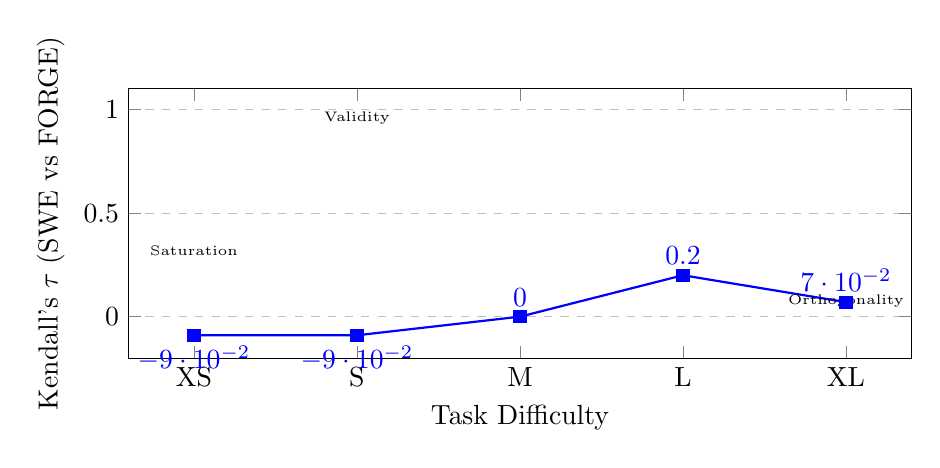
\begin{tikzpicture}
\begin{axis}[
    width=0.95\columnwidth,
    height=5cm,
    xlabel={Task Difficulty},
    ylabel={Kendall's $\tau$ (SWE vs FORGE)},
    symbolic x coords={XS, S, M, L, XL},
    xtick=data,
    ymin=-0.2, ymax=1.1,
    ymajorgrids=true,
    grid style=dashed,
    nodes near coords,
    point meta=y,
]
\addplot[color=blue, mark=square*, thick] coordinates {
    (XS,-0.09) % Saturation: Negative noise
    (S,-0.09)  % Validity: Weak correlation
    (M,0.00)  % Validity: Moderate correlation
    (L,0.20)  % Stability
    (XL,0.07) % Orthogonality: Inverse correlation!
};
\node [anchor=south] at (axis cs:XS,0.25) {\tiny Saturation};
\node [anchor=south] at (axis cs:S,0.88) {\tiny Validity};
\node [anchor=south] at (axis cs:XL,0.0) {\tiny Orthogonality};
\end{axis}
\end{tikzpicture}
\caption{The Benchmark Validity Window. The correlation turns negative for hard tasks (XL), because models with high static scores often crash, while robust models survive.}
\label{fig:validity-window}
\end{figure}

\begin{figure}[t]
\centering
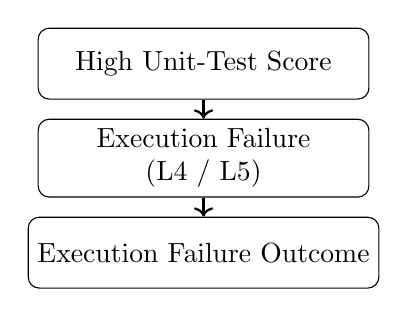
\begin{tikzpicture}[
  every node/.style={
    draw,
    rectangle,
    rounded corners,
    align=center,
    minimum width=4.2cm,
    minimum height=0.9cm
  },
  arrow/.style={->, thick}
]

\node (score) at (0,2.4) {High Unit-Test Score};
\node (fail)  at (0,1.2) {Execution Failure\\(L4 / L5)};
\node (out)   at (0,0)   {Execution Failure Outcome};

\draw[arrow] (score) -- (fail);
\draw[arrow] (fail) -- (out);

\end{tikzpicture}
\caption{Why failures matter. If the program crashes, it doesn't matter how good the code was—it's still a failure.}
\label{fig:failure-dominance}
\end{figure}

This section elucidates our findings through fundamental principles, examining the critical role of failures and their implications for AI evaluation.

\subsection{Failure Dominance and Ranking Reversal}
The data indicates a substantial divergence between traditional rankings and FORGE rankings. As shown in Table~\ref{tab:ranking-comparison}, results from simple code benchmarks and real-world execution differ significantly. For instance, GPT-5.2 scores high on static tests but ranks lower in FORGE, whereas Qwen3-Coder performs markedly better in this context. It appears that runtime crashes (L4/L5) negate gains from correct code snippets.

\subsection{Execution Failures as Blocking States}
We characterize execution failures (L4 and L5) as "blocking states." Once a system encounters one of these failures, operation ceases. At that point, the quality of the remaining code becomes irrelevant. Table~\ref{tab:overall-performance} indicates that models susceptible to these failures consistently achieve lower scores. This accounts for the observation that a model may be proficient at answering coding questions but deficient in building a working project: it repeatedly encounters these blocking states.

\subsection{Implications for Real-World Engineering Evaluation}
These failures highlight a disparity between "correct code" and "working systems." Models that perform well on simple tests often lack the capabilities to maintain a complex project. Conversely, models that avoid crashes tend to perform consistently well, even if their code is not flawless.

This suggests that execution testing is necessary to identify failures that simple tests overlook. Ultimately, verification of code snippets is insufficient to determine if an AI can construct reliable software.

\section{Failure Taxonomy}
\begin{figure}[t]
\centering
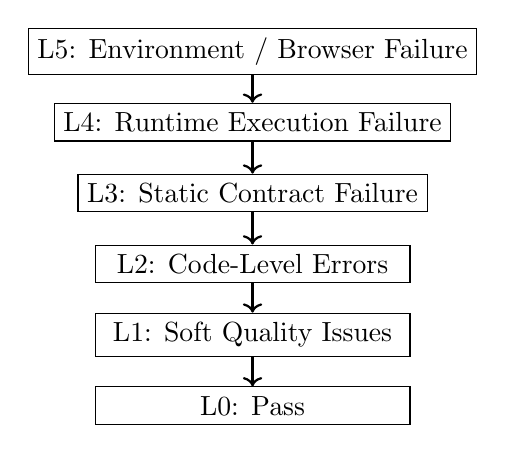
\begin{tikzpicture}[
  node distance=0.9cm,
  every node/.style={draw, rectangle, align=center, minimum width=4cm},
  arrow/.style={->, thick}
]
\node (l5) {L5: Environment / Browser Failure};
\node (l4) [below of=l5] {L4: Runtime Execution Failure};
\node (l3) [below of=l4] {L3: Static Contract Failure};
\node (l2) [below of=l3] {L2: Code-Level Errors};
\node (l1) [below of=l2] {L1: Soft Quality Issues};
\node (l0) [below of=l1] {L0: Pass};

\draw[arrow] (l5) -- (l4);
\draw[arrow] (l4) -- (l3);
\draw[arrow] (l3) -- (l2);
\draw[arrow] (l2) -- (l1);
\draw[arrow] (l1) -- (l0);
\end{tikzpicture}
\caption{Failure taxonomy with causal ordering. Higher layers dominate lower layers and override aggregate scores.}
\label{fig:failure-taxonomy}
\end{figure}

FORGE establishes a layered failure taxonomy classifying execution outcomes by \emph{causal priority} rather than severity.
Each layer corresponds to a distinct failure signal observed during static checks or execution.
Higher-layer failures supersede lower-layer signals and cannot be offset by partial correctness or aggregated scores.

\paragraph{L0 --- Non-failure / Pass.}
\textbf{Definition.}
Required artifacts are present, static checks are satisfied, and the project executes successfully without critical errors.

\textbf{Notes.}
Warnings, verbose logs, or ESG-related signals do not constitute failure.
L0 indicates the absence of observed failure, not necessarily optimal output.

\paragraph{L1 --- Soft Quality Issues.}
\textbf{Examples.}
Lint warnings (e.g., ESLint Level B or C), stylistic inconsistencies, unused innocuous code, or excessive logging.

\textbf{Characteristics.}
L1 signals do not impede execution and do not violate artifact validation rules.
They are recorded for analytical purposes but do not trigger failure.

\textbf{Key point.}
L1 signifies quality variance rather than functional failure.

\paragraph{L2 --- Code-Level Errors.}
\textbf{Examples.}
ESLint Level A errors, undefined variables, use-before-definition, or strictly logical errors.

\textbf{Characteristics.}
L2 comprises correctness errors detectable via static analysis.
Such errors may persist even if execution has not yet failed.

\textbf{Observation.}
L2 indicates that the program is inherently incorrect prior to execution.

\paragraph{L3 --- Static Contract Failure.}
\textbf{Examples.}
Missing requisite files, invalid JSON syntax, malformed HTML, or broken file linkages.

\textbf{Characteristics.}
L3 failures violate benchmark-level artifact protocols, precipitating failure independent of code quality.
They are not contingent upon the correctness of individual code blocks.

\textbf{Note.}
This layer captures a critical failure mode in project-based evaluation.

\paragraph{L4 --- Runtime Execution Failure.}
\textbf{Examples.}
Zero runtime score, essential sandbox startup failure, missing or invalid entry points, or unresponsive APIs.

\textbf{Characteristics.}
L4 failures indicate that the project is non-executable.
They supersede all static-level signals.

\paragraph{L5 --- Environment or Browser Failure.}
\textbf{Examples.}
Browser console errors, page-level runtime errors, network failures, or uncaught exceptions.

\textbf{Characteristics.}
L5 failures supersede all lower-level signals.
They are not mitigatable by static checks or runtime scores and are treated as definitive execution failures.

\paragraph{Causal Ordering Principle.}
The failure taxonomy adheres to a strict causal order:
environment failures override runtime execution failures, which override static contract failures, which override code-level correctness and quality issues.
This ordering prevents summary scores from obscuring fundamental execution breakdowns.

\section{Reproducibility and Transparency}

FORGE is designed to facilitate the reproducibility, inspection, and verification of evaluation results.
In lieu of reporting sole final scores, FORGE records execution procedures and runtime events.

\paragraph{Fixed Evaluation Rules.}
All task definitions, execution limits, scoring rules, and failure definitions are established prior to the commencement of evaluation.
These protocols are detailed herein and remain invariant throughout the evaluation process.
This prevents result-driven tuning and supports equitable comparison across models.

\paragraph{Executable and Replayable Runs.}
FORGE evaluates models via the execution of generated projects within process-isolated environments subject to essential sandboxing.
Execution is governed by explicit configuration files and command-line settings.
Execution logs capture runtime status, errors, and key context, enabling the replay of evaluations under identical conditions.

\paragraph{Model-level Records.}
In addition to summary scores, FORGE generates model-level records for each task.
These records encompass execution outcomes, assigned failure categories, and objective runtime metrics.
They preserve raw signals prior to aggregation, enabling the inspection of individual cases.

\paragraph{Transparent Statistics.}
All reported metrics and rankings adhere to documented procedures.
Aggregation methods, normalization steps, and ranking rules are explicitly defined.
Given model-level records, all statistics are recomputable without reliance on opaque processing.

\paragraph{Scope and Limits.}
In this context, reproducibility denotes the capacity to replay evaluations using identical protocols and configurations.
It does not guarantee identical low-level behavior across disparate hardware or systems.
FORGE prioritizes transparent evaluation logic and traceable results over hardware-specific determinism.


\section{Ethical and ESG Considerations}

FORGE constitutes an evaluation framework rather than a system for model training or deployment.
Consequently, ethical and ESG considerations focus on the design, reporting, and interpretation of evaluations, rather than on downstream model behavior.

\paragraph{Responsible Evaluation.}
Benchmarks may overestimate model capabilities when execution constraints are disregarded.
By evaluating runnable projects and prioritizing execution failures as primary signals, FORGE promotes a prudent interpretation of results.
To enhance the transparency of evaluation costs, we introduce the \textbf{Evaluation Compute Index (ECI)}:
$\mathrm{ECI} = (\texttt{parameterScale} \times \texttt{EvalToken}) / 10{,}000$.
ECI facilitates relative comparisons of evaluation-time compute usage.
For closed-source models lacking required data, ECI is reported as \texttt{Null}.

\paragraph{Environmental and Governance Considerations.}
Evaluation-time computation entails energy consumption and warrants responsible reporting.
By disclosing ECI, FORGE disincentivizes excessive computation for marginal performance gains.
FORGE further emphasizes auditability: evaluation rules are fixed before execution, execution traces are recorded, and summary reports document failure patterns.
ECI is designed as a comparative indicator rather than a precise measure of environmental impact, and the scope of FORGE is restricted to responsible evaluation practices.

\section{Limitations}

FORGE evaluates the behavior of generated projects during execution within controlled environments.
It is not intended to quantify all dimensions of model behavior, such as training data, internal reasoning, or long-term performance after deployment.
Consequently, FORGE should be interpreted as an evaluation of execution reliability, not as a comprehensive measure of model capability.

FORGE utilizes \textbf{Isolated Processes} and \textbf{Essential Sandboxing} to ensure equitable and repeatable evaluation.
These environments are static and controlled, yet represent simplified abstractions of production systems.
Alternative runtime configurations or infrastructure choices may expose additional failures that are not captured by the benchmark.
This represents a trade-off between realism and reproducibility.

The failure taxonomy in FORGE provides a structured perspective on common failure types, though it is not exhaustive.
Certain failure modes may remain unobserved within the current tasks or domains.
The taxonomy is designed for extension as new tasks and failure patterns emerge.

The tasks in FORGE encompass a subset of real-world software engineering activities.
They may exhibit bias towards specific project types or application domains.
Consequently, performance on FORGE should not be construed as a universal measure of software engineering ability.

The Evaluation Compute Index (ECI) serves as an approximate indicator of evaluation-time compute usage.
It does not quantify actual energy consumption and does not account for hardware efficiency or energy sources.
ECI is intended for relative comparison and transparency, not for precise environmental reporting.

Execution duration may fluctuate due to external API rate limits and queueing behavior that are outside the control of the FORGE system.
These effects introduce stochasticity rather than systematic bias and do not affect correctness, failure classification, or the relative robustness trends reported in this work.
Consequently, execution time rankings should be interpreted as contextual signals rather than strict performance measures.

Finally, FORGE results warrant careful interpretation.
Execution-intensive tasks and failure dominance rules may exacerbate discrepancies between models.
FORGE is not designed to supplant existing benchmarks, but to complement them by highlighting execution-related strengths and weaknesses.
These limitations indicate directions for future research rather than fundamental structural deficiencies.


\section{Conclusion}

This paper introduced FORGE, a novel framework for evaluating AI agents on real engineering tasks. Unlike prior benchmarks that focus on isolated code fragments, FORGE assesses an agent's ability to construct and execute a complete project.

Our results indicate that proficiency in generating code snippets is insufficient. Models that excel in unit tests often fail when constructing real systems due to fundamental errors such as missing artifacts or invalid dependencies. FORGE identifies these failures by evaluating every layer of the project, from code syntax to the runtime environment.

We designed FORGE to be open, fair, and accessible. By testing execution and tracking failures transparently, we can better understand the current limitations of AI. We hope that this work encourages the field to develop agents that not only generate code but also construct functional, reliable software.

% =========================
% References
% =========================
\bibliography{references}
\bibliographystyle{icml2026}

% =========================
% Appendix
% =========================
\newpage
\appendix
\onecolumn
\section{Supplementary Attachments Overview}

To support reproducibility, transparency, and independent verification, we provide a set of supplementary attachments.
All core definitions, evaluation protocols, and conclusions are fully contained in the main paper.
The attachments serve as supporting materials for reproducing experiments, inspecting execution behavior, and auditing failure and ESG-related analyses.

\paragraph{Attachment Directory.}
The supplementary materials are organized as follows:

\begin{itemize}
  \item \texttt{reproducibility.md}: Specifies the experimental environment, hardware and software dependencies, random seeds, and exact commands required to fully reproduce all FORGE benchmark runs.

  \item \texttt{failure-layer-taxonomy.md}: Defines the failure-layer taxonomy adopted by FORGE, including formal layer definitions, decision rules, and concrete execution-level examples.

  \item \texttt{stats-details.md}: Describes statistical aggregation procedures, scoring formulas, normalization rules, and ranking computation methods used to summarize benchmark results.

  \item \texttt{esg-disclaimer.md}: Clarifies the scope, assumptions, and explicit limitations of ESG-related considerations within the FORGE benchmark; no normative or compliance claims are made.

  \item \texttt{README.md}: Provides a high-level overview of the attachment directory, file organization, and navigation guidance for supplementary materials.

  \item \texttt{micro-reports/}: Contains model-specific post-execution evaluation artifacts, organized by model identifier (e.g., \texttt{gpt-5.2}, \texttt{grok-4}, \texttt{qwen3-coder}), including:
  \begin{itemize}
    \item \texttt{{modelname}/eval\_evaluation\_report.md / .json}: Per-model execution and evaluation summaries, including task outcomes and failure taxonomy statistics.
    \item \texttt{{modelname}/failure\_taxonomy\_report.md / .json}: Structured failure-layer breakdowns derived from execution traces.
    \item \texttt{{modelname}/esg\_evaluation\_report.md / .json}: ESG-related analytical reports derived from execution metadata (descriptive only).
    \item \texttt{README.md}: Documentation describing the structure, schema, and interpretation of the micro-report files.
  \end{itemize}
\end{itemize}

These materials enable reviewers and future researchers to replay executions, inspect failure behavior, and verify reported statistics without relying on undocumented assumptions.
All code, configurations, and experimental artifacts are provided to support transparent and repeatable evaluation.

\section{GITHUB-MIT Open Source}

The code for this project is available on GitHub under the MIT License at \url{https://github.com/Urcocra/forge}
\end{document}